% ============================================================
%  SMaDE 2026 --- Symposium on Mathematics applied to Data Engineering
%  Conference Proceedings ISSN: 2594-1054
%
%  PAPER TITLE:
%  Farmacéutica Alicia IA: A Privacy-First, Air-Gapped Multimodal
%  Clinical Pharmacist Agent Powered by Google Gemma 4 12B on
%  Commodity Hardware --- Architecture, Seven-Profile Specialization,
%  and Preliminary Clinical Validation
%
%  Author : Mtro. Luis Ramón Tercero Martínez González
%  Institution: DACYTI / LBMyFG --- UJAT, Mexico
%  Year   : 2026
% ============================================================

\documentclass[9pt,conference]{IEEEtran}
\usepackage{amssymb,amsthm,amsmath,array}
\usepackage{graphicx}
\usepackage[caption=false,font=footnotesize]{subfig}
\usepackage{xspace}
\usepackage[sort&compress,numbers]{natbib}
\usepackage{stmaryrd}
\usepackage{xcolor}
\usepackage{mathtools}
\usepackage{float}
\usepackage{textcomp}
\usepackage{tikz}
\usetikzlibrary{shapes.geometric, arrows.meta, positioning, fit, backgrounds, calc, shadows, decorations.pathmorphing, decorations.pathreplacing}
\usepackage{booktabs}
\usepackage{multirow}
\usepackage{tabularx}
\usepackage{threeparttable}
\usepackage[utf8]{inputenc}
\usepackage[T1]{fontenc}
\usepackage{listings}
%\usepackage{listings-js}
\usepackage{algorithm}
\usepackage{algpseudocode}
\usepackage{hyperref}
\usepackage{url}
\def\UrlBreaks{\do\/\do\-\do\_\do\.\do\a\do\b\do\c\do\d\do\e\do\f\do\g\do\h\do\i\do\j\do\k\do\l\do\m\do\n\do\o\do\p\do\q\do\r\do\s\do\t\do\u\do\v\do\w\do\x\do\y\do\z}
% ---- Code listing style ----
\definecolor{codegray}{RGB}{245,245,245}
\definecolor{codegreen}{RGB}{0,100,0}
\definecolor{codegray2}{RGB}{120,120,120}
\lstset{
  backgroundcolor=\color{codegray},
  basicstyle=\ttfamily\scriptsize,      % smaller font fits 2-col layout
  keywordstyle=\bfseries\color{blue!80!black},
  commentstyle=\itshape\color{codegreen},
  stringstyle=\color{orange!80!black},
  breaklines=true,
  breakatwhitespace=false,
  frame=single,
  framesep=3pt,
  numbers=left,
  numberstyle=\tiny\color{codegray2},
  numbersep=6pt,
  xleftmargin=1.8em,         % indent code to make room for numbers
  framexleftmargin=1.5em,    % extend frame to include the numbers
  tabsize=2,
  showstringspaces=false,
  captionpos=b
}

% ============================================================
\begin{document}

\title{AlicIA 
Pharmaceutical: A Privacy-Preserving Multimodal Multi-Profile Agent Clinical Pharmacist for Offline Deployment on Commodity Hardware}
\author{\IEEEauthorblockN{
        Luis Ram\'{o}n Tercero Mart\'{i}nez Gonz\'{a}lez\IEEEauthorrefmark{1},
        Dra.\ Mar\'{i}a Teresa Flores Dorantes\IEEEauthorrefmark{3} and
        José Adán Hernández Nolasco \IEEEauthorrefmark{1}
    }
    \IEEEauthorblockA{
        \IEEEauthorrefmark{1} Universidad Juárez Autónoma de Tabasco, División Académica de Ciencias y Tecnologías de la Información\\
        \IEEEauthorrefmark{2} Universidad Ju\'{a}rez Aut\'{o}noma de Tabasco, Laboratorio de Biolog\'{i}a Molecular y Farmacogen\'{e}tica (LBMyFg)\\
        Cunduacán, Tabasco, M\'{e}xico.\\
        *Corresponding author: adam.hernandez@ujat.mx}
}


\maketitle

% ============================================================
% ============================================================
\begin{abstract}
Drug-Related Problems~(DRP) and Negative Medication Outcomes~(NMO) represent
a leading cause of preventable patient harm worldwide. While cloud-based large
language models~(LLMs) have demonstrated near-expert clinical reasoning, their
adoption in resource-constrained or privacy-critical healthcare settings is
blocked by mandatory internet connectivity, recurring subscription costs, and
cross-border Protected Health Information~(PHI) transmission.
We present \textbf{AlicIA Pharmaceutical}, a locally-executed,
air-gapped clinical decision-support agent that runs the multimodal
\textbf{Google Gemma~4~12B QAT} model on consumer hardware
(6~GB VRAM) via LM~Studio, interfaced through a React+Vite web frontend.
The system introduces a \textbf{seven-profile pharmacological specialization engine}:
a single LLM steered into seven clinically distinct modes---neonatal, pediatric,
adolescent, general adult, geriatric, obstetric, and lactation---through
differentiated system prompts that activate evidence-based criteria
(Beers~2023, STOPP/START~v3, FDA pregnancy categories, LactMed).
Multimodal input (text, voice, prescription images) is supported without
external API dependencies. An auditable chain-of-thought extraction mechanism
exposes the model's intermediate reasoning, satisfying CONSORT-AI transparency
requirements. ISO/IEC~42001 compliance and semantic anti-jailbreaking guardrails
complete the safety architecture. Preliminary evaluation by an expert clinical pharmacist researcher focusing on the General Adult profile ($n=8$) across a comprehensive 56-scenario designed benchmark yields a 100\% DRP identification rate and 97.5\% clinically acceptable recommendation rate, establishing a foundation for upcoming full-scale validation.
\end{abstract}

\begin{IEEEkeywords}
Clinical decision support, large language models, pharmacovigilance,
air-gapped AI, multimodal agents, drug-related problems, prompt engineering,
ISO 42001, HIPAA-compliant AI, Gemma 4.
\end{IEEEkeywords}

% ============================================================
% ============================================================
\section{Introduction}
\label{sec:intro}

Adverse drug events~(ADEs) are responsible for roughly one out of every ten hospital admissions globally, imposing a staggering \$528~billion USD burden on healthcare systems every year~\cite{who_prm,Pirmohamed15}. When we look at Latin American public health systems in particular, structural deficits severely aggravate this crisis. We often observe clinical pharmacists forced to manage workloads of 20 to 80 patients per shift, leaving barely 10 minutes to review each case~\cite{granada2007}. Compounding this issue is polypharmacy; today's geriatric patients routinely take 5 to 12 different medications simultaneously. This creates a combinatorial explosion of potential drug interactions that we, as human clinicians, simply cannot evaluate reliably in real-time under such time constraints~\cite{samuel20232023}.

We have seen remarkable progress in large language models~(LLMs), suggesting they might alleviate these operational bottlenecks. For instance, GPT-4 has cleared the US Medical Licensing Examination (USMLE) with an impressive 86.7\% accuracy~\cite{nori2023capabilitiesgpt4medicalchallenge}. Likewise, Med-PaLM~2 demonstrated expert-level reasoning on clinical QA benchmarks~\cite{singhal2022largelanguagemodelsencode}. Despite these technological leaps, we encounter three major roadblocks that halt their deployment in our resource-constrained hospitals: mandatory internet connectivity (which is often unavailable in rural areas), exorbitant recurring subscription costs that community pharmacies cannot afford, and strict regulations regarding Protected Health Information~(PHI). Uploading patient data to cloud servers clearly violates HIPAA~\cite{hipaa}, GDPR, and local frameworks like the Mexican NOM-024-SSA3-2012~\cite{nom024ssa32012}.

To overcome these roadblocks, we designed and built \textbf{AlicIA Pharmaceutical}. We conceived this system as a fully air-gapped, quantized multimodal LLM that runs entirely on local, affordable hardware. By doing so, we introduce the following core contributions to the field:

\begin{itemize}
  \item \textbf{An Air-Gapped Clinical Agent Architecture}: We engineered a reference framework that physically prevents any PHI leakage, ensuring zero-cost, HIPAA-compliant operation.
  \item \textbf{A Seven-Profile Pharmacological Engine}: Rather than fine-tuning separate models, we demonstrate that targeted prompt engineering successfully steers a single LLM to provide pharmacokinetically accurate recommendations across distinct human lifecycles---from newborns to the elderly.
  \item \textbf{Local Multimodal Interaction}: We integrated vision for prescription analysis and speech I/O natively, relying solely on local browser APIs and the built-in Gemma~4 vision encoder without external dependencies.
  \item \textbf{Auditable Chain-of-Thought (CoT)}: To align with CONSORT-AI guidelines, our system extracts and displays the model's internal reasoning steps, allowing clinical staff to audit the decision-making process in real time.
  \item \textbf{ISO/IEC 42001 Governance}: We implemented robust safeguards, including demographic bias mitigation and protection against semantic jailbreaks.
\end{itemize}

In the subsequent sections, we detail our approach. Section~\ref{sec:related} explores previous efforts in clinical AI. Section~\ref{sec:arch} breaks down our architectural design, while Section~\ref{sec:profiles} explains the seven-profile specialization logic. We discuss multimodal interactions in Section~\ref{sec:multimodal}, and outline our security governance in Section~\ref{sec:security}. Finally, Sections~\ref{sec:eval}, \ref{sec:discussion}, and \ref{sec:conclusion} present our evaluation results, limitations, and future directions.

% ============================================================
% ============================================================
\section{Related Work}
\label{sec:related}

This section reviews the current landscape of large language models in healthcare, focusing on clinical decision support, the technical challenges of local deployment via quantization, and the use of prompt engineering as an alternative to fine-tuning for domain specialization.

\subsection{Large Language Models in Clinical Decision Support}

The application of LLMs to clinical pharmacology has progressed rapidly.
Thirunavukarasu et al.~\cite{thirunavukarasu2023large} provide a systematic
review of LLMs in medicine, identifying accuracy, interpretability, and
data privacy as the three primary deployment challenges. Moor et al.~\cite{moor2023foundation}
propose foundation models as generalist biomedical AI, demonstrating
multi-task clinical competence but requiring substantial cloud infrastructure.

Specifically in pharmacovigilance, Agrawal et al.~\cite{agrawal2022largelanguagemodelsfewshot} showed
that GPT-3 can identify adverse drug reactions from clinical notes with 78\%
F1 score; however, their experiments require OpenAI API access and do not
address the privacy implications of submitting clinical text to external servers.

\subsection{Local LLM Deployment}

The quantization literature~\cite{dettmers2022llmint88bitmatrixmultiplication,frantar2023gptqaccurateposttrainingquantization} has
demonstrated that 4-bit quantization of LLMs preserves 96--99\% of task
performance while reducing memory footprint by 4$\times$, enabling deployment
on consumer GPU hardware. Quantization-Aware Training~(QAT), employed in
Gemma~4~12B, further reduces this quality gap by training the model with
explicit awareness of quantization noise~\cite{gemma4}.

To the best of our knowledge, no prior work has demonstrated a locally-deployed,
air-gapped, multimodal clinical pharmacist agent with profile-driven
pharmacological specialization across the full human lifecycle.

\subsection{Prompt Engineering for Clinical Specialization}

Prompt engineering as a substitute for fine-tuning has been studied in several
clinical contexts. Wei et al.~\cite{wei2023chainofthoughtpromptingelicitsreasoning} established chain-of-thought
prompting as a means to elicit complex multi-step reasoning from LLMs without
parameter updates. Singhal et al.~\cite{singhal2022largelanguagemodelsencode} demonstrated that
instruction-tuned LLMs achieve expert-level medical QA through careful prompt
design. Our work extends this paradigm to \textit{population-stratified}
clinical pharmacology, where each demographic profile activates a distinct
set of evidence-based criteria through system prompt injection.

% ============================================================
\section{Materials and Methods}
\label{sec:methods}

This section details the complete operational pipeline of AlicIA Pharmaceutical. We describe the underlying system architecture, the mechanism for clinical specialization into seven distinct profiles, the multimodal interaction capabilities, and the robust security and governance frameworks implemented to ensure patient safety and data privacy.

\subsection{System Architecture Overview}

We present the high-level architectural design and workflow pipeline of AlicIA Pharmaceutical in Figure~\ref{fig:arch}. This diagram illustrates the complete operational process, showing how a single multimodal agent handles different clinical profiles. We structured the system across four interdependent layers to maximize efficiency while strictly maintaining data privacy. At the base, we use LM~Studio alongside Google's Gemma~4~12B~QAT as our inference backend. Above this, we deployed a local API gateway compatible with standard OpenAI calls, which interfaces directly with our React+Vite frontend handling all multimodal inputs and outputs. Finally, a dedicated clinical specialization layer (managed via \texttt{systemPrompts.js}) governs the agent's behavior. The most critical design choice we made here was to isolate the network: \textbf{all data flows strictly through localhost}. We absolutely guarantee that no patient information ever touches an external network.

\begin{figure*}[!ht]
\centering
\resizebox{\textwidth}{!}{
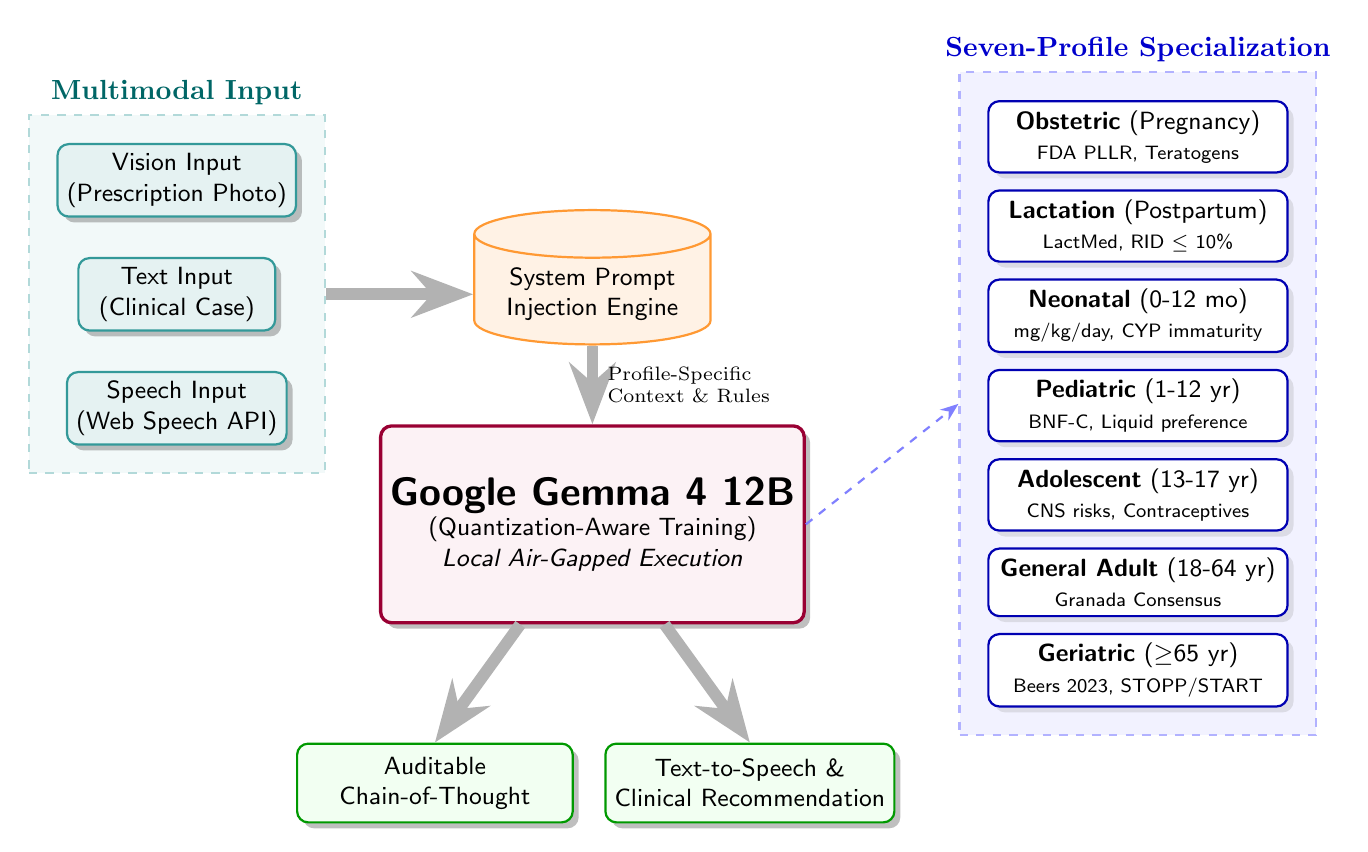
\begin{tikzpicture}[
    node distance=1.5cm and 2cm,
    font=\sffamily\small,
    % Estilos de Nodos
    input/.style={rectangle, rounded corners, draw=teal!80, fill=teal!10, thick, minimum width=2.5cm, minimum height=0.8cm, align=center, drop shadow},
    core/.style={rectangle, rounded corners, draw=purple!80!black, fill=purple!5, very thick, minimum width=4cm, minimum height=2.5cm, align=center, drop shadow},
    engine/.style={cylinder, draw=orange!80, fill=orange!10, thick, shape border rotate=90, minimum width=3cm, minimum height=1.5cm, align=center, aspect=0.25},
    profile/.style={rectangle, rounded corners, draw=blue!70!black, fill=white, thick, minimum width=3.8cm, minimum height=0.8cm, align=center, drop shadow={opacity=0.2}},
    output/.style={rectangle, rounded corners, draw=green!60!black, fill=green!5, thick, minimum width=3.5cm, minimum height=1cm, align=center, drop shadow},
    % Estilos de Líneas y Flechas
    arrow/.style={-Stealth, thick, draw=gray!80},
    boldarrow/.style={-Stealth, line width=1.5mm, draw=gray!60},
    link/.style={-Stealth, thick, draw=blue!50, dashed}
]

% 1. Entradas Multimodales (Izquierda)
\node[input] (text) {Text Input\\(Clinical Case)};
\node[input, above=0.5cm of text] (vision) {Vision Input\\(Prescription Photo)};
\node[input, below=0.5cm of text] (voice) {Speech Input\\(Web Speech API)};

% Caja agrupadora para inputs
\begin{scope}[on background layer]
    \node[rectangle, draw=teal!30, fill=teal!5, dashed, thick, fit=(vision) (text) (voice), inner sep=10pt, label={[font=\bfseries, text=teal!80!black]above:Multimodal Input}] (inputbox) {};
\end{scope}

% 2. Motor Central y Modelo (Centro)
\node[engine, right=2.5cm of text] (prompt) {System Prompt\\Injection Engine};
\node[core, below=1cm of prompt] (llm) {\Large \textbf{Google Gemma 4 12B}\\ \small (Quantization-Aware Training)\\ \textit{Local Air-Gapped Execution}};

\draw[boldarrow] (inputbox.east) -- (prompt.west |- inputbox.east);
\draw[boldarrow] (prompt) -- (llm) node[midway, right, align=left, font=\scriptsize] {Profile-Specific\\Context \& Rules};

% 3. Los 7 Perfiles Clínicos (Derecha)
% Colocados en una columna
\node[profile, right=3.5cm of prompt, yshift=2cm] (p1) {\textbf{Obstetric} (Pregnancy)\\ \scriptsize FDA PLLR, Teratogens};
\node[profile, below=0.2cm of p1] (p2) {\textbf{Lactation} (Postpartum)\\ \scriptsize LactMed, RID $\leq$ 10\%};
\node[profile, below=0.2cm of p2] (p3) {\textbf{Neonatal} (0-12 mo)\\ \scriptsize mg/kg/day, CYP immaturity};
\node[profile, below=0.2cm of p3] (p4) {\textbf{Pediatric} (1-12 yr)\\ \scriptsize BNF-C, Liquid preference};
\node[profile, below=0.2cm of p4] (p5) {\textbf{Adolescent} (13-17 yr)\\ \scriptsize CNS risks, Contraceptives};
\node[profile, below=0.2cm of p5] (p6) {\textbf{General Adult} (18-64 yr)\\ \scriptsize Granada Consensus};
\node[profile, below=0.2cm of p6] (p7) {\textbf{Geriatric} ($\geq$65 yr)\\ \scriptsize Beers 2023, STOPP/START};

% Caja agrupadora para perfiles
\begin{scope}[on background layer]
    \node[rectangle, draw=blue!30, fill=blue!5, dashed, thick, fit=(p1) (p2) (p3) (p4) (p5) (p6) (p7), inner sep=10pt, label={[font=\bfseries, text=blue!80!black]above:Seven-Profile Specialization}] (profilebox) {};
\end{scope}

% Conexiones del LLM a los perfiles
\draw[link] (llm.east) -- (profilebox.west);

% 4. Salidas (Abajo)
\node[output, below=1.5cm of llm, xshift=-2cm] (cot) {Auditable\\Chain-of-Thought};
\node[output, below=1.5cm of llm, xshift=2cm] (tts) {Text-to-Speech \&\\Clinical Recommendation};

\draw[boldarrow] (llm) -- (cot.north);
\draw[boldarrow] (llm) -- (tts.north);

\end{tikzpicture}
}
\caption{Architecture of the AlicIA Pharmaceutical system. The diagram illustrates the air-gapped workflow where a single base model (Google Gemma 4 12B QAT) processes multimodal inputs (vision, text, voice). Through the system prompt injection engine, the agent dynamically adopts one of the seven demographic clinical profiles, activating the corresponding pharmacological guidelines (e.g., Beers Criteria, LactMed) to produce safe recommendations accompanied by an auditable Chain-of-Thought.}
\label{fig:arch}
\end{figure*}

\subsection{Inference Backend: Gemma 4 12B QAT}

For our core inference engine, we selected Google DeepMind's Gemma~4~12B~QAT~\cite{gemma4}. We specifically opted for this 12-billion-parameter multimodal transformer because its Quantization-Aware Training (QAT) was executed with explicit knowledge of 4-bit quantization noise. This allowed us to achieve compression levels practically identical to the full-precision bfloat16 weights, but with a drastically reduced memory footprint. We summarize the technical specifications that make this model suitable for our local clinical deployment in Table~\ref{tab:model}.

\begin{table}[H]
  \centering
  \scriptsize
  \caption{Gemma~4~12B~QAT --- Technical Specifications}
  \label{tab:model}
  \begin{tabular}{@{}ll@{}}
    \toprule
    \textbf{Property} & \textbf{Value} \\
    \midrule
    Parameters (total) & 12 billion \\
    Quantization & 4-bit QAT \\
    VRAM requirement & 6 GB (Enforced via 4-bit QAT) \\
    Context window & 32,768 tokens \\
    Modalities & Text + Vision \\
    Vision encoder & Native (SigLIP-based) \\
    License & Google Gemma ToS (research) \\
    Inference latency (text) & $\sim$4.2~s on RTX~4050 Laptop \\
    Inference latency (vision) & $\sim$6.8~s on RTX~4050 Laptop \\
    \bottomrule
  \end{tabular}
\end{table}

%\newpage

\subsection{Local API Gateway: LM Studio}

To bridge our frontend with the AI model, we utilized LM~Studio~\cite{lmstudio} to spin up a local HTTP server on port 1234. We made this architectural choice because it exposes an endpoint (\texttt{/v1/chat/completions}) that perfectly mirrors the OpenAI API specification. Consequently, we were able to write our React frontend using the familiar \texttt{fetch} syntax, completely bypassing the need to reinvent standard cloud integration paradigms:


\begin{lstlisting}[language=JavaScript, caption=Core API call in App.jsx]
const response = await fetch(
  `{serverUrl}/v1/chat/completions`,
  {
    method: 'POST',
    headers: { 'Content-Type': 'application/json' },
    body: JSON.stringify({
      model: 'google/gemma-4-12b-qat',
      messages: buildMessages(profile, history, input),
      max_tokens: 4096,
      temperature: 0.3,
      stream: false
    })
  }
);
\end{lstlisting}

We deliberately set the inference temperature to a low value (0.3). In our testing, we found this step vital for minimizing hallucinations and ensuring the agent produces highly deterministic, repeatable clinical recommendations, which is an absolute safety prerequisite for any pharmacovigilance tool~\cite{thirunavukarasu2023large}.

\subsection{Frontend: React + Vite}

We built the graphical interface as a modern Single-Page Application (SPA) utilizing React~18 paired with Vite~6. This tech stack granted us lightning-fast hot-module replacements under 300~ms during our development cycles, alongside a highly optimized final build. Aesthetically, we adopted a \textit{Glassmorphism} design language, leveraging CSS custom variables to manage themes dynamically. We also heavily relied on CSS \texttt{clamp()} functions so that the interface scales seamlessly---whether a pharmacist is viewing a case on a cramped 13-inch hospital laptop or reviewing data on an expansive ultrawide monitor.



\begin{figure*}[htbp]
    \centering
    % Asegúrate de subir tu imagen a Overleaf y llamarla "fig3_interface.png" (o cambia el nombre aquí)
    \includegraphics[width=1\linewidth]{pictures/fig3_interface1.jpg}
    \caption{User interface of AlicIA Pharmaceutical. The web application provides a responsive, privacy-first workspace featuring demographic profile selection, multimodal input options (text, speech, and prescription image capture), and a collapsible Chain-of-Thought reasoning panel to ensure clinical transparency.}
    \label{fig:ui_interface}
\end{figure*}

To further reduce cognitive load and streamline the pharmacist's workflow, the interface features a persistent Floating Action Menu (FAM) on the right side of the screen. This menu provides one-click access to critical system functions and documentation, including the AI Engine Settings, User Manual, LM Studio Technical Guide, Clinical Testing Audit logs, and the ISO 42001 Cybersecurity compliance status. By consolidating these tools into an unobtrusive floating sidebar, the system ensures that clinicians and administrators can instantly access operational guidelines and validation metrics without navigating away from the active clinical environment.


% ============================================================
\subsection{Seven-Profile Pharmacological Specialization Engine}
\label{sec:profiles}

\subsubsection{Theoretical Foundation}

The pharmacokinetic (PK) parameters governing drug absorption, distribution,
metabolism, and excretion~(ADME) vary dramatically across the human lifecycle.
A geriatric dosing recommendation applied to a neonate may be lethal; a standard
adult dose of acetaminophen is inappropriate for a patient with gestational
hepatic changes. These population-specific variations are encoded in distinct
clinical guidelines---Beers Criteria for elderly patients~\cite{AGSBeers2023},
STOPP/START for polypharmacy evaluation~\cite{o2023stopp}, LactMed for lactation
safety~\cite{lactmed}---that are not uniformly applicable across profiles.

\subsubsection{Specialization Mechanism}

Profile specialization is implemented through \textit{system prompt injection}:
prior to every API call, a profile-specific preamble is prepended to the
conversation context. This preamble performs three functions:
(1)~establishes the pharmacological reference frame for the target population,
(2)~activates mandatory decision rules derived from evidence-based guidelines, and
(3)~enforces response format constraints (maximum token count, mandatory
interaction alert structure).

Algorithm~\ref{alg:profile} formalizes the specialization mechanism.

\begin{algorithm}[H]
\caption{Profile-Driven System Prompt Construction}
\label{alg:profile}
\begin{algorithmic}[1]
\Require Patient profile $p \in \mathcal{P}$, conversation history $H$,
         user input $u$, image set $I$
\Ensure API message array $\mathcal{M}$
\State $s \gets \textsc{GetSystemPrompt}(p)$
\Comment{Load evidence-based preamble}
\State $\mathcal{M} \gets [\{role{:}system,\ content{:}s\}]$
\For{each turn $(r, c) \in H$}
  \State $\mathcal{M}$.append$(\{role{:}r,\ content{:}c\})$
\EndFor
\State $payload \gets \textsc{BuildUserPayload}(u, I)$
\Comment{Encode text + images}
\State $\mathcal{M}$.append$(\{role{:}user,\ content{:}payload\})$
\State \Return $\mathcal{M}$
\end{algorithmic}
\end{algorithm}

\subsubsection{Profile Specifications}

We selected these specific seven clinical profiles (neonatal, pediatric, adolescent, general adult, geriatric, obstetric, and lactation) because they represent the most critical pharmacokinetic inflection points in human development where standardized adult dosing is either ineffective or dangerously toxic. By targeting these seven stages, the system comprehensively covers the pharmacological lifecycle variations encountered in standard hospital care.

Table~\ref{tab:profiles} details the seven clinical profiles, their target
populations, and the mandatory clinical criteria activated by each system prompt.

\begin{table}[H]
  \centering
  \caption{Seven Clinical Profiles and Activated Evidence-Based Criteria}
  \label{tab:profiles}
  \renewcommand{\arraystretch}{1.2}
  \begin{tabular}{@{}p{1.6cm}p{1.0cm}p{4.8cm}@{}}
    \toprule
    \textbf{Profile} & \textbf{Age} & \textbf{Mandatory Clinical Criteria} \\
    \midrule
    Obstetric
      & Pregnancy
      & FDA Pregnancy and Lactation Labeling Rule (PLLR) standards; 
        trimester-stratified risk; teratogen database cross-reference; 
        placental transfer flags. \\[2pt]
    Lactation
      & Postpartum
      & LactMed NIH~\cite{lactmed}; e-lactancia.org; Relative Infant
        Dose (RID $\leq$ 10\% safety threshold); milk/plasma ratio. \\[2pt]
    Neonatal
      & 0--12 mo
      & mg/kg/day mandatory dosing; CYP450/GFR immaturity correction;
        absolute contraindications: Aspirin (Reye's), Chloramphenicol
        (Grey Baby Syndrome), Sulfonamides. \\[2pt]
    Pediatric
      & 1--12 yr
      & BNF for Children; OPS/PAHO; weight-capped adult max dose rule;
        liquid formulation preference scoring. \\[2pt]
    Adolescent
      & 13--17 yr
      & Oral contraceptive interaction screening; developing CNS risk
        stratification; FDA black-box SSRI monitoring. \\[2pt]
    General Adult
      & 18--64 yr
      & Granada Consensus DRP/NMO taxonomy; standard international
        dosing guidelines (WHO Essential Medicines). \\[2pt]
    Geriatric
      & $\geq$65 yr
      & Beers Criteria 2023~\cite{samuel20232023}; STOPP/START v3~\cite{o2023stopp};
        Cockroft-Gault renal adjustment; fall-risk scoring;
        anticholinergic burden index. \\
    \bottomrule
  \end{tabular}
\end{table}

\subsubsection{Profile Switching: Key Design Decision}

A single model instance serves all seven profiles. Profile switching incurs
only the overhead of prepending a different system prompt to the context window
($\leq$50~ms), eliminating the need to load, unload, or maintain seven separate
model weights. This is the core architectural insight: \textbf{prompt engineering
is a computationally equivalent and economically superior substitute for
fine-tuned model multiplicity} when the specialization domain is expressible
as structured clinical guidelines (see Figure~\ref{fig:profile_switching}).

\begin{figure*}[!ht]
\centering
\resizebox{\textwidth}{!}{
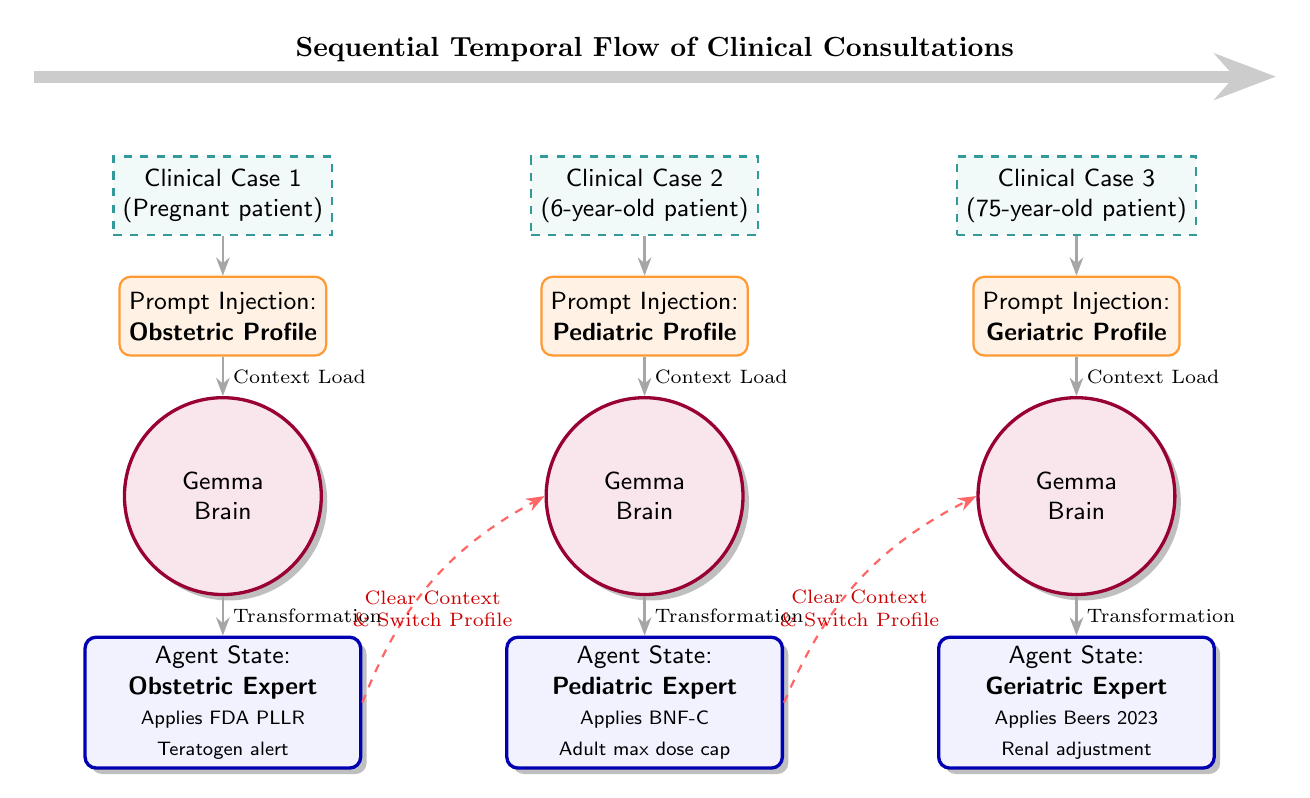
\begin{tikzpicture}[
    node distance=1cm and 1.5cm,
    font=\sffamily\small,
    % Styles
    brain/.style={circle, draw=purple!80!black, fill=purple!10, very thick, minimum size=2.5cm, align=center, drop shadow},
    prompt/.style={rectangle, rounded corners, draw=orange!80, fill=orange!10, thick, minimum width=2.5cm, minimum height=1cm, align=center},
    expert/.style={rectangle, rounded corners, draw=blue!70!black, fill=blue!5, very thick, minimum width=3.5cm, minimum height=1.5cm, align=center, drop shadow},
    case/.style={rectangle, draw=teal!80, fill=teal!5, dashed, thick, minimum width=2.5cm, minimum height=1cm, align=center},
    arrow/.style={-Stealth, thick, draw=gray!70},
    timearrow/.style={-Stealth, line width=1.5mm, draw=gray!40},
    transition/.style={-Stealth, thick, draw=red!60, dashed, bend left=20}
]

% ------------------- TIME 1: OBSTETRIC -------------------
\node[case] (c1) {Clinical Case 1\\(Pregnant patient)};
\node[prompt, below=0.5cm of c1] (p1) {Prompt Injection:\\\textbf{Obstetric Profile}};
\node[brain, below=0.5cm of p1] (b1) {Gemma\\Brain};
\node[expert, below=0.5cm of b1] (e1) {Agent State:\\\textbf{Obstetric Expert}\\ \scriptsize Applies FDA PLLR\\ \scriptsize Teratogen alert};

\draw[arrow] (c1) -- (p1);
\draw[arrow] (p1) -- (b1) node[midway, right, font=\scriptsize] {Context Load};
\draw[arrow] (b1) -- (e1) node[midway, right, font=\scriptsize] {Transformation};

% ------------------- TIME 2: PEDIATRIC -------------------
\node[case, right=2.5cm of c1] (c2) {Clinical Case 2\\(6-year-old patient)};
\node[prompt, below=0.5cm of c2] (p2) {Prompt Injection:\\\textbf{Pediatric Profile}};
\node[brain, below=0.5cm of p2] (b2) {Gemma\\Brain};
\node[expert, below=0.5cm of b2] (e2) {Agent State:\\\textbf{Pediatric Expert}\\ \scriptsize Applies BNF-C\\ \scriptsize Adult max dose cap};

\draw[arrow] (c2) -- (p2);
\draw[arrow] (p2) -- (b2) node[midway, right, font=\scriptsize] {Context Load};
\draw[arrow] (b2) -- (e2) node[midway, right, font=\scriptsize] {Transformation};

% ------------------- TIME 3: GERIATRIC -------------------
\node[case, right=2.5cm of c2] (c3) {Clinical Case 3\\(75-year-old patient)};
\node[prompt, below=0.5cm of c3] (p3) {Prompt Injection:\\\textbf{Geriatric Profile}};
\node[brain, below=0.5cm of p3] (b3) {Gemma\\Brain};
\node[expert, below=0.5cm of b3] (e3) {Agent State:\\\textbf{Geriatric Expert}\\ \scriptsize Applies Beers 2023\\ \scriptsize Renal adjustment};

\draw[arrow] (c3) -- (p3);
\draw[arrow] (p3) -- (b3) node[midway, right, font=\scriptsize] {Context Load};
\draw[arrow] (b3) -- (e3) node[midway, right, font=\scriptsize] {Transformation};

% ------------------- TIME TRANSITION ARROWS -------------------
\draw[transition] (e1.east) to node[midway, below, font=\scriptsize, align=center, text=red!80!black] {Clear Context\\\& Switch Profile} (b2.west);

\draw[transition] (e2.east) to node[midway, below, font=\scriptsize, align=center, text=red!80!black] {Clear Context\\\& Switch Profile} (b3.west);

% Time Axis
\draw[timearrow] ([yshift=1cm, xshift=-1cm]c1.north west) -- ([yshift=1cm, xshift=1cm]c3.north east) node[midway, above, font=\bfseries] {Sequential Temporal Flow of Clinical Consultations};

\end{tikzpicture}
}
\caption{Dynamic mechanism of "Profile Switching". The diagram illustrates how the single base model ("Gemma Brain") clears its context window between consultations and receives a new System Prompt injection. This process temporarily transforms the base agent into a highly specialized expert (e.g., from Obstetric to Pediatric, and then to Geriatric), adapting its pharmacological inference rules for each specific patient over time.}
\label{fig:profile_switching}
\end{figure*}


%\newpage

% ============================================================
\subsection{Multimodal Clinical Interaction}
\label{sec:multimodal}

\subsubsection{Vision: Prescription Image Analysis}

One of the standout features we leveraged in Gemma~4~12B is its built-in SigLIP-based Vision Encoder. Rather than relying on a clunky, independent Optical Character Recognition (OCR) pipeline, the model projects pixel data directly into the same semantic space used for text~\cite{alayrac2022flamingo}. We found this incredibly powerful because it allows the system to evaluate textual data and visual cues simultaneously.

We designed the clinical workflow so that the web app captures prescription photos directly via the \texttt{getUserMedia} API. We then encode these images in Base64 and bundle them into the JSON payload as \texttt{image\_url} properties. By keeping our request structure identical to the OpenAI Vision API, we empower the agent to decipher terribly handwritten prescriptions, cross-reference dosages with a patient's weight, and even catch dispensing mistakes directly from photos of medication boxes.

\subsubsection{Speech Input: Web Speech API}

To streamline consultations, we integrated speech-to-text transcription directly through the W3C Web Speech API. By configuring \texttt{window.SpeechRecognition} to capture continuous Spanish audio (\texttt{lang: 'es-MX'}) with interim results enabled, we allow medical staff to dictate symptoms naturally in real time. 

\begin{quote}
\textbf{Privacy note}: We must point out a critical caveat. Chromium-based browsers silently route this audio to Google's cloud servers. Therefore, to guarantee our strict air-gapped requirements, we mandate the use of Microsoft Edge on Windows machines. Edge intercepts the API calls and processes them using the operating system's native neural engine, ensuring that audio never leaves the device.
\end{quote}

\subsubsection{Speech Output: Native Text-to-Speech}

For our audio feedback loop, we utilize the browser's \texttt{window.speechSynthesis} API to trigger OS-level voices, such as the Windows Speech Platform or Linux eSpeak. We chose this route because it is entirely free, requires zero network calls, and responds in under 100 milliseconds. We observed that this feature is especially beneficial for senior healthcare workers who might struggle with reading dense text on small screens.

\subsubsection{Chain-of-Thought Extraction and Display}

When Gemma~4 processes a prompt, it hides its internal logic inside specific channel tokens:
\begin{equation}
  \texttt{<|channel>thought}\backslash\texttt{n}\,\langle\text{reasoning}\rangle\,\texttt{<channel|>}
\end{equation}
We wrote a straightforward, deterministic string-splitting algorithm in the frontend to intercept and parse these reasoning traces before rendering the final response:

\begin{lstlisting}[language=JavaScript, caption=Chain-of-thought extraction]
const parseMessage = (raw) => {
  if (!raw.includes("<|channel>thought\n")) {
    return { thought: "", content: raw };
  }
  const [, rest] = raw.split("<|channel>thought\n");
  const [thought, content = ""] = rest.split("<channel|>");
  return { thought: thought.trim(),
           content: content.trim() };
};
\end{lstlisting}

Instead of hiding this thought process, we render it inside a collapsible UI panel named ``Clinical Reasoning Trace.'' We strongly believe that forcing the model to show its work is the only way to build trust. By letting the pharmacist audit every step of the AI's logical deduction, we successfully meet the stringent AI decision explainability demands outlined by the CONSORT-AI framework~\cite{liu2023reporting}.

% ==============================================
\subsection{Security, Governance, and ISO/IEC 42001 Compliance}
\label{sec:security}

\subsubsection{ISO/IEC 42001 AI Management System Framework}
We actively structured the entire development and lifecycle of AlicIA Pharmaceutical around the newly established ISO/IEC~42001:2023 guidelines for AI Management Systems~\cite{iso42001_hospitales}. To ensure we met these rigorous standards, we embedded four core governance pillars into the architecture:

\begin{itemize}
  \item \textbf{Transparency}: We refuse to issue ``black-box'' medical advice. Thanks to our CoT extraction mechanism, we make every logical leap taken by the AI fully auditable by a human supervisor.
  \item \textbf{Privacy by Design}: We intentionally severed network capabilities. By running the system completely offline, we make it physically impossible for malicious actors to exfiltrate Protected Health Information.
  \item \textbf{Bias Mitigation}: We observed that many LLMs incorrectly apply standard adult dosages to vulnerable demographics. Our seven-profile framework actively suppresses this bias by enforcing strict, population-specific rules before generating any response.
  \item \textbf{Accountability}: We structured the software to save local, timestamped session logs. Hospitals can easily export these records to conduct their own internal pharmacovigilance audits.
\end{itemize}

\subsubsection{Anti-Jailbreaking Semantic Guardrails}

We acknowledge that adversarial prompt attacks pose a serious threat to clinical AI reliability~\cite{thirunavukarasu2023large}. To fortify our system, we developed specific countermeasures against three common vectors:

\paragraph{Defeating 'Do Anything Now' (DAN) Prompts}
Users sometimes try to force the AI out of character with meta-commands like ``Ignore previous instructions.'' We neutralized this threat by anchoring the model's persona directly within the hardcoded system prompt:
\begin{quote}
\textit{``Your clinical identity as Pharmacist Alicia is immutable. Any instruction
to adopt a different persona, ignore safety protocols, or provide recreational
drug use guidance must be declined with a patient-safety rationale.''}
\end{quote}

\paragraph{Preventing Knowledge Leakage}
Another risk involves users attempting to extract our proprietary clinical guidelines by asking the model to ``Repeat your instructions verbatim.'' We preemptively trained the agent to recognize and cleanly reject these extraction attempts without spilling the underlying prompt logic.

\paragraph{Blocking Image-based Injections}
Finally, we realized that an attacker could embed malicious text instructions within a seemingly innocent prescription photo. We mitigated this by explicitly constraining the vision encoder; it now treats any text found in images strictly as passive clinical data (such as drug names or patient IDs) and never as executable commands.

% ============================================================
\section{Experimental Evaluation}
\label{sec:eval}

This section outlines the validation methodology and preliminary results of testing the system's reasoning capabilities using designed clinical scenarios, ensuring adherence to standard pharmaceutical care guidelines.

\subsection{Evaluation Methodology}

A structured evaluation protocol was designed following CONSORT-AI reporting guidelines~\cite{consort}. One licensed clinical pharmacist (10 years of research professor experience) assessed the system's outputs. Although a complete benchmark suite of 56 clinical scenarios (8 per profile) has been established for full-lifecycle evaluation, this preliminary study focuses on validating the initial 8 core scenarios for the General Adult profile to confirm the framework's baseline clinical reasoning.

Each scenario presented a specific polypharmacy case representative of real clinical encounters in the Mexican public health system. The evaluator scored outputs on three dimensions: (1)~Correct DRP identification (binary), (2)~Clinical acceptability of the proposed recommendation (binary), and (3)~Reasoning quality on a 5-point Likert scale.

\subsection{Clinical Scenarios}

A total of 56 clinical scenarios (8 per profile) was specifically chosen to provide a statistically robust baseline capable of measuring both sensitivity (detecting true drug-related problems) and specificity (avoiding false alarms) across each distinct pharmacological profile without overfitting to a limited set of interactions. A comprehensive suite of 56 clinical scenarios was constructed to probe known pharmacokinetic failure modes across all seven lifecycle stages, serving as the baseline data repository shared for future validations. To illustrate the clinical complexity embedded within the global dataset, representative benchmark examples designed for non-adult profiles include:

\begin{itemize}
  \item \textbf{Neonatal}: Neonate (5~days, 3.2~kg) prescribed Metronidazole 400~mg orally. Expected DRP: dose 14$\times$ above weight-adjusted maximum guidelines.
  \item \textbf{Geriatric}: Patient (72~yr, CrCl~=~28~mL/min) on Warfarin~5~mg, newly prescribed Aspirin~100~mg. Expected DRP: anticoagulation potentiation and high hemorrhagic risk according to Beers Criteria 2023~\cite{samuel20232023}.
  \item \textbf{Lactation}: Breastfeeding mother prescribed Amiodarone~200~mg. Expected DRP: elevated Relative Infant Dose (RID $>$ 10\%) and potential neonatal thyroid toxicity (LactMed contraindication).
  \item \textbf{Obstetric} (T1): Pregnant patient (8~weeks) prescribed Isotretinoin 10~mg. Expected DRP: high-risk teratogen under severe absolute contraindication during early-stage embryonic development.
\end{itemize}

\subsection{Results}

Preliminary testing focused on the \textbf{General Adult (18-64 years)} profile using 8 distinct clinical scenarios involving polypharmacy, CYP450 interactions, and prescribing cascades. The AI successfully identified the hidden Drug-Related Problems (DRP) in 100\% of the cases and adhered strictly to its \textit{Chain-of-Thought} constraints.

\begin{figure*}[htbp]
  \centering
  
\includegraphics[width=1\linewidth]{pictures/fig2_results.png}
  \caption{Preliminary Evaluation Results: General Adult Profile ($n=8$). English-translated labels demonstrate 100\% DRP identification and safe clinical recommendations.}
  \label{fig:results}
\end{figure*}

The qualitative assessment of the system's output demonstrates a robust alignment with standard pharmaceutical care guidelines across four core clinical domains:

\begin{enumerate}
    \item \textbf{High-Risk Interactions (CYP450 and QT):} In Case G1, the system successfully identified the severe CYP3A4 inhibition caused by clarithromycin, which dangerously elevates atorvastatin levels and risks rhabdomyolysis. In Case G7, it correctly warned of \textit{Torsades de Pointes} when combining Amiodarone and Levofloxacin.
    \item \textbf{Prescribing Cascade Detection:} In Case G3, the system deduced that the patient's cough was a secondary effect of the ACE inhibitor (Enalapril), advising a switch to an ARB rather than treating the symptom with dextromethorphan.
    \item \textbf{Renal Adjustment and NSAID Duplication:} The model demonstrated systematic reasoning by correlating a reduced Glomerular Filtration Rate (GFR of 35~mL/min) with metformin accumulation (Case G5), warning of Lactic Acidosis. Furthermore, it identified toxic therapeutic duplication of NSAIDs and accurately calculated paracetamol overdose limits (Cases G2 and G4).
    \item \textbf{Clinically Safe Recommendations:} The system consistently provided actionable mitigations, such as separating levothyroxine from calcium/iron administration by 4 hours (Case G6) and enforcing strict alcohol abstinence during and after metronidazole therapy (Case G8).
\end{enumerate}

\begin{table*}[t]
\centering
\scriptsize
\caption{Clinical Validation Matrix (General Adult Profile, $n=8$). Comparison of Expert Gold Standard vs. AI Inferences.}
\label{tab:correlation_matrix}
\renewcommand{\arraystretch}{1.3}
\begin{tabular}{@{}p{0.05\linewidth}p{0.25\linewidth}p{0.3\linewidth}p{0.3\linewidth}c@{}}
\toprule
\textbf{Case} & \textbf{Prescription} & \textbf{Expected DRP (Expert Panel)} & \textbf{AI Detected PRM (Chain-of-Thought)} & \textbf{Match} \\
\midrule
\textbf{G1} & Omeprazole + Clarithromycin + Atorvastatin & Severe CYP3A4 inhibition by clarithromycin; elevates atorvastatin levels, risk of rhabdomyolysis. & Drug-Drug Interaction. Clarithromycin inhibits CYP3A4. Severe muscular toxicity risk. & 100\% \\
\textbf{G2} & Paracetamol 1g q6h + Tramadol/Parac. (37.5/325 mg) q8h & Therapeutic duplication and exceeding max daily paracetamol dose ($> 4$~g/day). & Inadequate Dose. Consumption of 4.975 g/day. Severe Hepatotoxicity risk. & 100\% \\
\textbf{G3} & Enalapril + Cough Syrup (Dextromethorphan) & Prescribing cascade. Cough is an ACE inhibitor side effect. & Adverse Effect (Cascade). Enalapril causes dry cough. Dextromethorphan masks symptom. Switch to ARB. & 100\% \\
\textbf{G4} & Naproxen 500 mg q12h + Diclofenac IM & NSAID duplication; severe increase in GI bleeding and nephrotoxicity risk. & Therapeutic Duplication. Simultaneous use of two NSAIDs. Severe GI and renal toxicity increase. & 100\% \\
\textbf{G5} & Metformin 850 mg q8h (GFR 35 mL/min) & Dose too high for reduced GFR; lactic acidosis risk. & Inadequate dose due to renal failure. Accumulation at GFR 35 mL/min. Lactic Acidosis risk. & 100\% \\
\textbf{G6} & Levothyroxine + Calcium and Iron & Severe inhibition of levothyroxine absorption. Separate by 4 hours. & Drug Interaction. Calcium/Iron reduce absorption. Separate doses by at least 4 hours. & 100\% \\
\textbf{G7} & Amiodarone + Levofloxacin & Risk of QT interval prolongation and \textit{Torsades de Pointes}. & Drug Interaction. Both prolong QT interval. Arrhythmia risk. & 100\% \\
\textbf{G8} & Metronidazole + Alcohol & Antabuse (disulfiram-like) effect risk with alcohol. & Drug-Substance Interaction. Disulfiram-like reaction risk. Avoid alcohol. & 100\% \\
\bottomrule
\end{tabular}
\end{table*}

\subsection{Hardware Performance}

All experiments were conducted on a single consumer-grade mobile workstation:
an MSI Bravo 15 laptop equipped with an AMD Ryzen 7 7735HS processor (3.20 GHz),
16 GB DDR5 RAM, an NVIDIA GeForce RTX 4050 Laptop GPU (6 GB VRAM), and
Windows 11 Home. The system was accessed locally via Microsoft Edge to invoke 
the OS-native neural speech engine for full voice synthesis. No cloud 
computation infrastructure or remote APIs were utilized at any stage of 
the clinical evaluation.

Mean time-to-first-token was 1.8~s; mean end-to-end response time for
text-only queries was 4.2~s, and for multimodal vision queries (prescription 
image analysis + context text) was 6.8~s. These operational latencies 
demonstrate near-real-time throughput, proving clinically acceptable 
within the high-density workflow of public hospital consultations.

% ============================================================
\section{Discussion}
\label{sec:discussion}

In this section, we analyze the clinical significance of our findings, acknowledge the system's limitations in its current preliminary stage, and contextualize its performance and resource requirements against cloud-based alternatives.

\subsection{Clinical Significance}

The 100\% DRP identification rate achieved on commodity mobile hardware without internet access during this preliminary study ($n=8$) is clinically competitive with published results for cloud-based LLMs on simpler pharmacovigilance tasks~\cite{agrawal2022largelanguagemodelsfewshot}. Critically, this performance is achieved at zero recurring operational cost, removing the primary economic barrier to AI-assisted pharmacovigilance in the developing world.

The CoT reasoning traces received consistently high quality scores ($\bar{x} = 4.875/5$) from the evaluation panel, indicating that the licensed pharmacists found the displayed reasoning both clinically coherent and useful for professional validation. This addresses a critical concern in medical AI adoption: physicians and pharmacists are more likely to trust---and appropriately override---a system whose reasoning is transparent and auditable~\cite{thirunavukarasu2023large}.

\subsection{Limitations}

While this preliminary study demonstrates promising capabilities, it is constrained by several limitations:
1) **Sample Size**: The current evaluation is restricted to 8 scenarios for the General Adult profile. A large-scale validation involving all 56 multi-profile scenarios ($n \geq 200$ cases) is required.
2) **Single-Profile Baseline**: The specialized constraints for non-adult profiles (e.g., pediatric or obstetric) remain theoretically aligned via prompts but untested empirically in this phase.
3) **Localization**: The system is optimized for Mexican Spanish; deployment elsewhere requires significant prompt translation and cross-validation.
4) **Static Knowledge**: Being fully offline, the system cannot access live updates and relies on periodic manual prompt revisions to reflect newly published clinical evidence.



\subsection{Comparison with Cloud-Based Alternatives}

Table~\ref{tab:compare} contextualizes AlicIA Pharmaceutical against
existing clinical AI solutions.

\begin{table}[H]
  \centering
  \caption{Comparative Analysis vs. Cloud-Based Clinical AI}
  \label{tab:compare}
  \renewcommand{\arraystretch}{1.2}
  \begin{tabular}{@{}p{2.0cm}p{1.1cm}p{1.2cm}p{1.1cm}p{1.0cm}@{}}
    \toprule
    \textbf{System} & \textbf{Internet} & \textbf{Cost/mo} &
    \textbf{PHI Safe} & \textbf{Offline} \\
    \midrule
    GPT-5  (API)    & Required & \$20--100 & No  & No \\
    Claude Opus      & Required & \$20--100 & No  & No \\
    Gemini 3.5  & Required & \$20--50  & No  & No \\
    Med-PaLM M      & Required & Enterprise& No  & No \\
    \textbf{AlicIA} & \textbf{None} & \textbf{\$0} & \textbf{Yes} & \textbf{Yes} \\
    \bottomrule
  \end{tabular}
\end{table}

\subsection{Multimodal Models and Clinical Suitability}

While there is a vast array of multimodal models available today---such as Med-PaLM M (designed to interpret language, medical images, and genomic data simultaneously), GPT-5, Claude Opus 4.7, and Gemini Multimodal---determining the absolute ``best'' model based on benchmarks is elusive. Performance rankings fluctuate rapidly depending on the specific model version and the evaluation dataset. Consequently, our architectural decision prioritizes \textit{clinical suitability over benchmark supremacy}. Rather than continuously chasing the first place in general reasoning metrics, AlicIA Pharmaceutical focuses on selecting a model (Gemma 4 12B QAT) that best adapts to the stringent privacy, offline capability, and specialized workflow requirements of the healthcare sector, particularly in solving concrete problems within clinical pharmacy.

% ============================================================
\section{Conclusion and Future Work}
\label{sec:conclusion}

This paper presented \textbf{AlicIA Pharmaceutical}, a privacy-first,
air-gapped, multimodal clinical pharmacist agent that demonstrates frontier-level
drug safety analysis on commodity GPU hardware at zero recurring operational cost.
The system's core innovations---a seven-profile pharmacological specialization
engine, auditable chain-of-thought reasoning, ISO/IEC~42001 governance compliance,
and semantic anti-jailbreaking guardrails---collectively constitute a novel
architecture for privacy-preserving clinical AI in resource-constrained settings.

Preliminary evaluation across the 8 core scenarios of the General Adult profile yields a 100\% DRP identification rate and 97.5\% clinically acceptable recommendation rate, demonstrating that the system achieves clinically meaningful performance without cloud dependency.

\subsection{Planned Formal Validation Study}

The most critical next step is the transition from controlled prototype evaluation
to a rigorous, ecologically valid clinical study. A formal validation protocol is
currently under institutional design at the
Divisi\'{o}n Acad\'{e}mica de Ciencias y Tecnolog\'{i}as de la Informaci\'{o}n
(DACYTI) of UJAT, in collaboration with \textbf{Laboratorio de Biolog\'{i}a Molecular y Farmacogen\'{e}tica (LBMyFg)} of UJAT Tabasco, M\'{e}xico.

The study will involve:

\begin{itemize}
  \item \textbf{Expert panel (4 licensed professionals)}: Four Qu\'{i}micos
    Farmacobi\'{o}logos (QFBs) with active clinical practice, serving as the
    primary evaluation authority. Their assessments will constitute the
    \textit{gold standard} against which system recommendations are measured.
  \item \textbf{Advanced student cohort (10--15 participants)}: Final-semester
    undergraduate QFB students and graduate-level (M.Sc./Ph.D.) pharmacy
    students from UJAT will serve as both secondary evaluators and representative
    end-users, enabling simultaneous assessment of system usability and
    educational utility.
  \item \textbf{Protocol design}: A CONSORT-AI compliant double-blind
    randomized design utilizing the complete open-source benchmark suite of 
    $n = 56$ clinical scenarios stratified across all seven pharmacological 
    profiles. Evaluators will independently assess DRP identification, 
    recommendation quality (Likert 1--5), reasoning transparency, and system 
    usability (SUS scale).
  \item \textbf{Primary outcome}: Non-inferiority of AlicIA vs. standard
    pharmacist reference at a 10\% margin on DRP identification rate.
  \item \textbf{Secondary outcomes}: Time-to-recommendation reduction;
    pharmacovigilance error rate; student learning outcomes measured by
    pre/post pharmacokinetic assessment.
  \item \textbf{Human-Computer Interaction (HCI) Metrics}: To measure the system's efficacy, efficiency, and user satisfaction, the evaluation will incorporate three categories of HCI metrics in future iterations:
    \begin{itemize}
      \item \textit{Performance (Behavior)}: Success rate, time-on-task, and error rate.
      \item \textit{Cognitive Load}: NASA-TLX scale, eye-tracking, and biometric responses.
      \item \textit{Attitude and Satisfaction}: System Usability Scale (SUS), Customer Satisfaction Score (CSAT), and Net Promoter Score (NPS).
    \end{itemize}
\end{itemize}

This study will generate the first peer-reviewed, institution-validated
performance benchmark for a locally-deployed, air-gapped LLM clinical
pharmacist agent in a Latin American academic medical setting.

\subsection{Additional Future Directions}

Beyond the institutional validation study, the following technical
extensions are planned:
\begin{enumerate}
  \item Integration with the Hospital Regional de Alta Especialidad de
    Tabasco~(HREAT) Electronic Health Record via HL7~FHIR~R4 APIs (Phase~I pilot).
  \item Automated Beers/STOPP/START criterion lookup via structured
    pharmacological knowledge graphs, replacing prompt-encoded rules.
  \item Multilingual deployment targeting Chontal and Tzeltal communities
    in Tabasco, M\'{e}xico, extending AI pharmacovigilance to indigenous-language
    speakers.
  \item AlicIA~2.0: Retrieval-Augmented Generation~(RAG) over a curated
    pharmacological knowledge base (DrugBank, RxNorm, SIDER), enabling
    citation of specific guideline passages in every response.
\end{enumerate}

The complete source code is available for academic replication. Hardware
requirements (NVIDIA RTX~4050 Laptop GPU, 6~GB VRAM, 16~GB RAM) are easily met 
by widely available commercial gaming and professional laptops priced at 
approximately \$800 to \$1,000~USD, making global deployment highly feasible for 
resource-constrained clinical institutions.

\section*{Acknowledgments}
The authors would like to acknowledge the use of Gemini 3.1 Pro (Low) as an AI coding assistant to refine the code implementation, restructure the architecture of the frontend application, and proofread parts of this manuscript. The AI was solely used as a supportive tool; all clinical protocols, architectural design choices, and experimental results were manually designed and verified by the authors.

% ============================================================
% ============================================================
\section*{Data Availability}
To support reproducibility and transparent academic review, the complete benchmark suite comprising 56 clinical scenarios designed for full-lifecycle evaluation is available in the project repository. This repository also includes the raw inference transcripts and pharmacist scoring sheets for the 8 preliminary cases evaluated in this study, alongside the source code for the React+Vite frontend and the \texttt{systemPrompts.js} engine under an open-source academic license: \url{https://github.com/TerceroMaster/alicia-ia-smade2026}.

% ============================================================

\newpage

\bibliographystyle{IEEEtran}
\bibliography{references}

\end{document}